\documentclass[]{article}

\usepackage[utf8]{inputenc}
\usepackage[T1]{fontenc}
\usepackage[french]{babel}

\usepackage{hyperref}
\usepackage{nameref}

\usepackage{mathtools}
\usepackage{mathrsfs}


\usepackage{graphicx}
\usepackage{float}
\usepackage{lscape}
\usepackage{wrapfig}
\usepackage{rotating}

\usepackage{fullpage}

\usepackage{xcolor}
\usepackage{listings}
\usepackage{fixltx2e}

\definecolor{darkblue}{rgb}{0.0,0.0,0.6}
\definecolor{darkred}{rgb}{0.3,0.0,0.0}

\lstset{%
	breaklines=true,
	columns=fullflexible,
	showstringspaces=false
}

\lstdefinelanguage{XML}
{%
	morestring=[b]",
	morestring=[s]{>}{<},
	morestring=[s]{"}{"},
	moredelim=[s][\color{black}]{>}{<},
	stringstyle=\color{darkred},
	identifierstyle=\color{purple},
	keywordstyle=\color{darkblue},
	morekeywords={number, name, difficulty, maxTime, dependency, width, height, xPos, yPos, rotation, canBeMoved, canBeRotated}
}

\begin{document}

\title{Rapport d'analyse\\
	Projet de structures de données II\\
	\smallskip
	{\small Activité d'Apprentissage \textsf{S-INFO-020}}\\
}
\author{
Membres du groupe:\\
LABEEUW Dorian (\texttt{dorian.labeeuw@student.umons.ac.be}) \and JOERTZ Jonathan (\texttt{jonathan.joertz@student.umons.ac.be})}

\date{Année Académique 2017-2018\\
Bachelier en Sciences Informatiques Bloc 3\\ 
\vspace{1cm}
Faculté des Sciences, Université de Mons}

\maketitle

\medskip
\begin{center} \today \end{center}
	\begin{abstract}
		Ce \emph{rapport d'analyse} est rendu dans le cadre de l'AA \textsf{S-INFO-020} "Projet de structures de données II", dispensé par le professeur \emph{Bruyère Véronique} en année académique 2017-2018.
	\end{abstract}

\newpage

\tableofcontents

\newpage

\section{Énoncé du problème}
Dans le cadre de ce projet, nous devons comprendre et implémenter une solution au problème de \emph{map overlay} selon un article de recherche fourni. L'utilité de ce problème est de retrouver l'ensemble des points d'intersections d'un ensemble de segments donné. Afin de réussir une implémentation efficace (on entend par là que l'on recherche une solution meilleure que la solution naïve en \mathscr{O}($n^{2}$)), il nous est nécessaire d'utiliser 2 structures de données expliquées ci-après (voir \nameref{sub:mainQDesc} et \nameref{sub:mainTDesc}) et 3 algorithmes dont nous fournissons aussi une explication plus loin dans ce rapport (voir \nameref{sub:findInter}, \nameref{sub:eventPoint} et \nameref{sub:findNew}). De plus, certains cas poseront problème, nous donnons ici une brève explication de la façon dont nous avons prévu de les gérer (voir \nameref{sub:horiz} et \nameref{sub:interSeg}). Une des applications du problème de \emph{map overlay} se retrouve dans les cartes informatisées ou les \emph{GPS}.

\section{Description des structures de données}\label{sec:mainDesc}
    \subsection{Description de \mathcal{Q}}\label{sub:mainQDesc}
        \subsubsection{Description}\label{subsub:QDesc}
            \paragraph{} \mathscr{Q} est une \emph{event queue} stockée dans un arbre binaire de recherche balancé sans doublons dont l'ordre correspond à un \nameref{subsub:QOrd} défini plus loin. Les éléments stockés dans un noeud de \mathscr{Q} sont un point d'évènement et tous les segments commençant en ce point. 
            \paragraph{} Les 3 opérations que \mathscr{Q} doit supporter sont la suppression, la recherche du minimum et l'insertion sans doublons.
            \paragraph{} \mathscr{Q} sera sans doublons car on ne veut traiter qu'une seule fois un point d'évènement.
            \paragraph{} La complexité des algorithmes d'insertion et de suppression (et par extension de recherche) peuvent et doivent être implémentés en O(log(m)) où m est le nombre de noeuds présents dans \mathscr{Q}.
            \paragraph{} Le nombre de noeuds de \mathscr{Q} est plus petit que $s + i$ où s est le nombre de segments et i le nombre d'intersections. Ceci est le pire cas, en effet, ce cas-là apparait si tous les \emph{upper endpoints} (points de début des segments) sont au-dessus de la sweep line, si aucun \emph{lower endpoint} n'est au-dessus d'elle et si chaque segment ne croise que ses voisins et pas les segments plus loin.
        \subsubsection{Exemple}\label{subsub:QEx}
        
            \begin{center}
            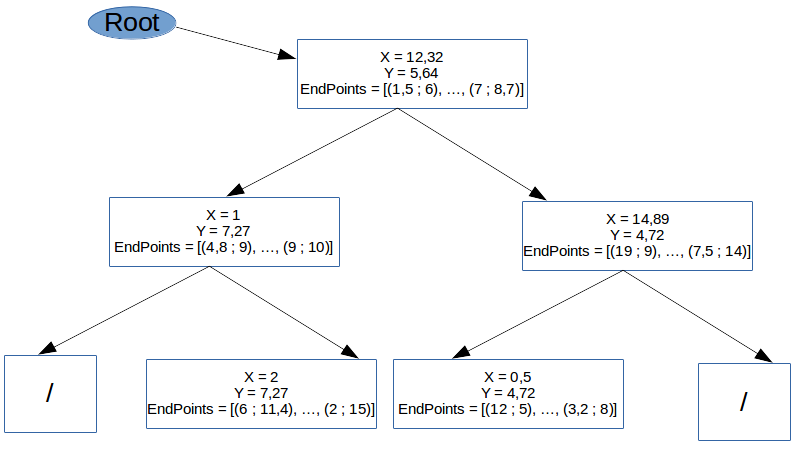
\includegraphics[width=15cm]{ExempleQPng}
            \end{center}
        \subsubsection{Ordre sous-jacent}\label{subsub:QOrd}
            \paragraph{} L'ordre est défini par le symbole $\prec$. Supposons que p et q sont deux points d'évènement. Alors on a $p \prec q \leftrightarrow (p\textsubscript{y} > q\textsubscript{y}) \vee (p\textsubscript{y} = q\textsubscript{y} \wedge p\textsubscript{x} < q\textsubscript{x})$.
            \paragraph{} Le cas particulier des \emph{segments horizontaux} se gère sans ajout particulier. En effet, le point gauche du segment sera considéré comme devant celui de droite.
        
    \subsection{Description de \mathscr{T}}\label{sub:mainTDesc}
        \subsubsection{Description}\label{subsub:TDesc}
        
        \subsubsection{Exemple}\label{subsub:TEx}
            \begin{center}
            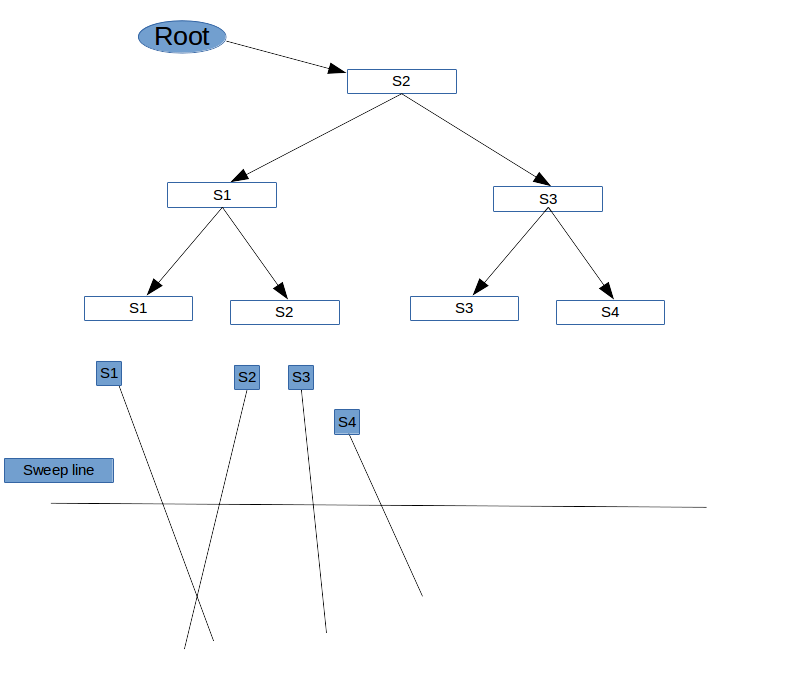
\includegraphics[width=15cm]{ExempleTPng}
            \end{center}
        \subsubsection{Ordre sous-jacent}\label{subsub:TOrd}

\section{Explication des algorithmes présentés}\label{sec:algos}
    \subsection{Explication de \emph{FindIntersections(S)}}\label{sub:findInter}
    
    \subsection{Explication de \emph{HandleEventPoint(p)}}\label{sub:eventPoint}
    
    \subsection{Explication de \emph{FindNewEvent(s\textsubscript{l}, s\textsubscript{r}, p)}}\label{sub:findNew}

\section{Gestion des cas particuliers}\label{sec:part}
    \subsection{Gestion des segments horizontaux}\label{sub:horiz}
    
    \subsection{Gestion des points d'intersection à au moins 3 segments}\label{sub:interSeg}

\section{Description des étapes du programme}\label{sec:prog}
%ATTENTION À MENTIONNER LES STRUCTURES UTILISÉES!!!

\end{document}
